\documentclass[utf8]{article}
\usepackage[utf8]{inputenc}
\usepackage{hyperref}
\usepackage{graphicx}
\title{Assignment 1 - Group 18}
\author{Henry Yang, Erik Karlkvist \\Jesper Jaxing, Oskar Willman\\ Zoe Sanderson-Wall, Danielle Santos\\Alexander Håkansson}
\date{November 3 - 2016}
\begin{document}
	\maketitle
	\section{what is a good team member?}
	\begin{itemize}
		\item Be on schedule
		\item Bring muffin (fika?)
		\item If given a Task, they shall complete it, and if not able to, communicate it in time. (and ask for help if necessary).
		\item Tell your team what you are doing. - Be responsible for making the rest of the team understand your work.
	\end{itemize}
	\subsection{What should a good team member NOT do!}
	\begin{itemize}
		\item Not judge the others, if they are not doing fine.
		\item Take the credit for someone else's work.
		\item Not over shun people.
	\end{itemize}
	\section{Goals and Objectives}
	Aim for our highest respective grades (5 or VG) and try NOT to miss it. This is a collective objectives.
	After completing the course We are expecting to be able to:
	\begin{itemize}
		\item Knowledge and understanding
		\item describe how models can be used for design and analysis of a software system
		\item describe how models can be used for specifying the behavior of a software system
		\item summarize how models can be used for documenting software systems
		\item illustrate how models can fit into a software process consisting of analysis, design and implementation
	\end{itemize}
	\section{Brief Description of the Project context}
	We are suppose to make a booking system for a hotel, that focuses on checking in and checking out, book hotel room, and basic managing tools for the Hotel staff (e.g. Manager and receptionists).
	\\Use cases ar defined \href{https://pingpong.chalmers.se/courseId/7502/node.do?id=3369884}{here}.

	\section{Domain model of the hotel domain}
	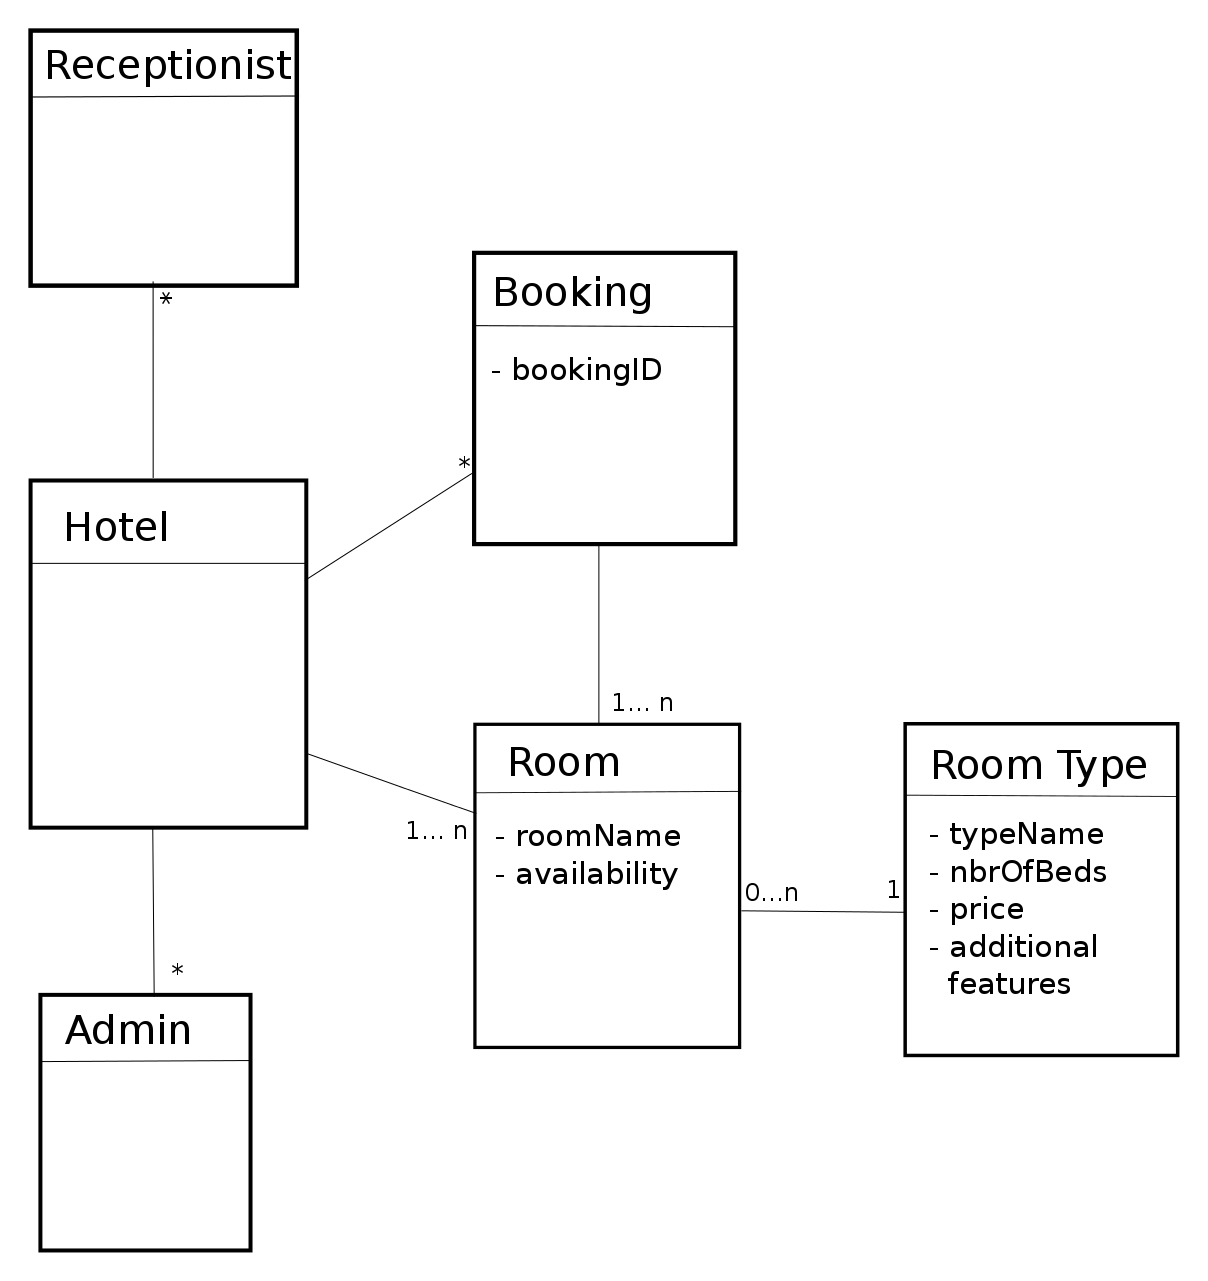
\includegraphics[scale=0.2]{ClassDiagram}
	\section{Use case diagram, created in Papyrus, which reflects the entire requirements specification}
	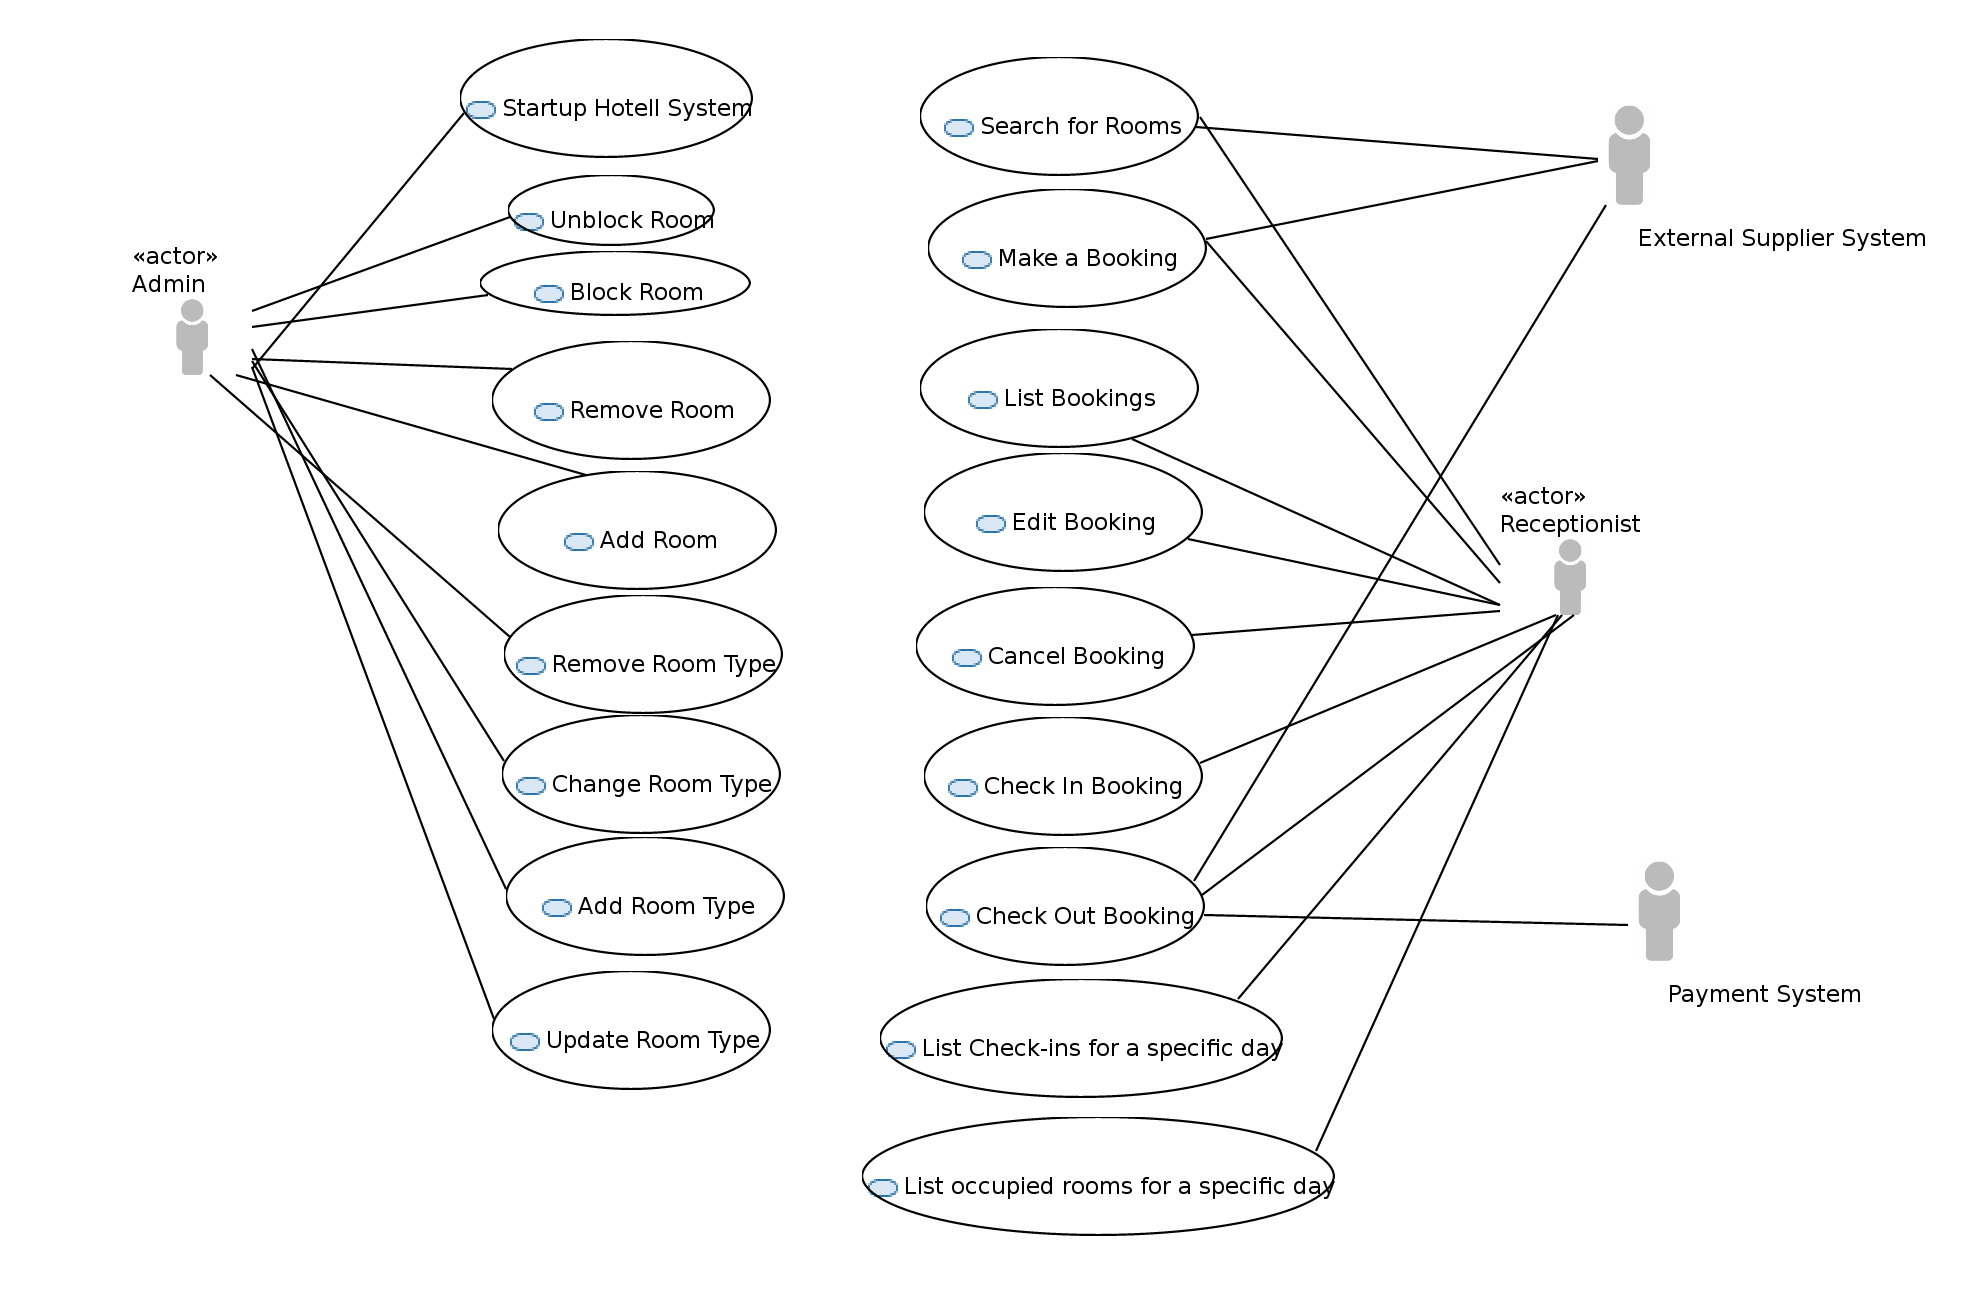
\includegraphics[scale=0.2]{use-case-diagram}
	\subsection{Link to repository}
	The URL to our repository can be found here:\\
	\url{https://github.com/Jaxing/TDA593-18}
\end{document}
